
\subsection{Exponential Decay}\label{ex:decay-set-sample}

We would like to demonstrate the qualitative differences in the solutions provided by the set-- and sample--based methods for a nonlinear problem.
To this end, we consider the exponential decay problem with uncertain decay rate and initial condition (which are paired to form the 2-D vector $\param$):
$$
\begin{cases}
  \frac{\partial u}{\partial t} & = \param_1 u(t), \\
  u(0) &= \param_2.
\end{cases}
$$

The solution is described by
\begin{equation}
  u(t;\param) = u_0\exp(\param_1 t), \; u_0 = \param_2 ,
\end{equation}

and a nominal value of $\param = 0.5$ is used to simulate the system.
We take a single observation at $t=0.5$s and assume a uniform density with interval length $0.2$ centered at $u(1,0.5)$ to represent the uncertainty in the measurement equipment.
We assume a uniform ansatz / initial density over the unit domain.
We use $N=50$ parameter samples to establish a coarse solution in Figure~\ref{fig:heatrod-sol-ex1}.


\begin{figure}
\begin{minipage}{.475\textwidth}
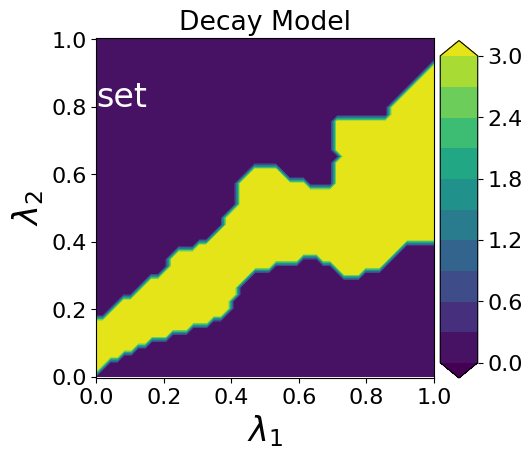
\includegraphics[width=\linewidth]{examples/fig_decay_q1/DecayModel--set_N50_em.png}
\end{minipage}
\begin{minipage}{.475\textwidth}
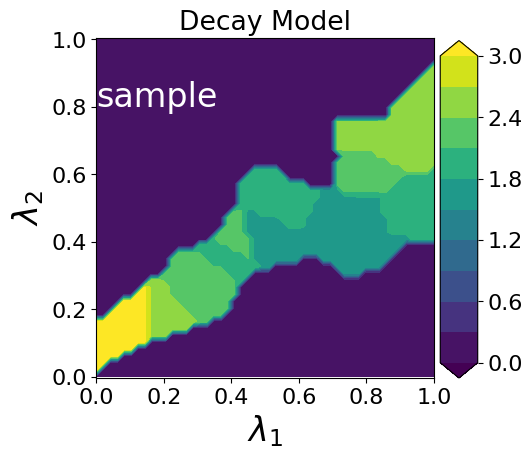
\includegraphics[width=\linewidth]{examples/fig_decay_q1/DecayModel--sample_N50_mc.png}
\end{minipage}
\caption{Observation taken at $t=1$s. The inverse image of the reference measure for set-based (left) and sample-based (right) solutions for $\nsamps=50$ parameter samples.}
\label{fig:heatrod-sol-ex1}
\end{figure}

The decay rate $\param_1$ shows little reduction in uncertainty overall.
If one were to look at marginals of the components of $\param$, it would not appear as if much was learned.
However, the relationship \emph{between} these two quantities has very certainly been elucidated by the solution of the inverse problem.
Where once $\pspace$ was a rectangular region, the set of possible parameters has been reduced to a diagonal band.
The sample-based approach, especially at this low sample size (density estimation in 2-D at $50$ samples is a stretch), has some visible downsides.
It does not capture the equivalence--class nature of the solution set the way the set--valued one does, which benefits from using $\ndiscs=1$ (aligning with the choice of uniform observed density).


We address what would occur had we been able to observe earlier in time, say at $t=0.5$ by showing the associated solutions under the same experimental conditions in \ref{fig:heatrod-sol-ex2}.
There is a marked reduction in uncertainty, as several regions of $\pspace$ have been ruled out from consideration.


\begin{figure}
\begin{minipage}{.475\textwidth}
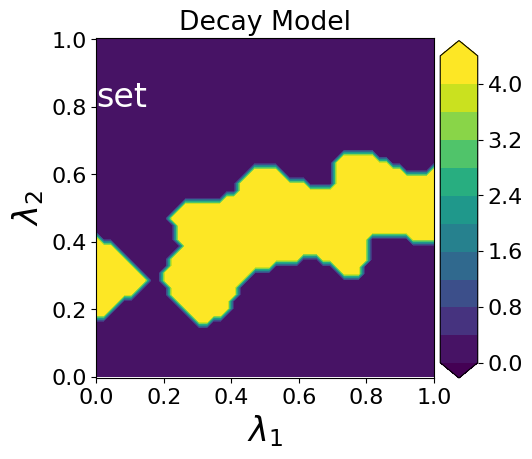
\includegraphics[width=\linewidth]{examples/fig_decay_q2/DecayModel--set_N50_em.png}
\end{minipage}
\begin{minipage}{.475\textwidth}
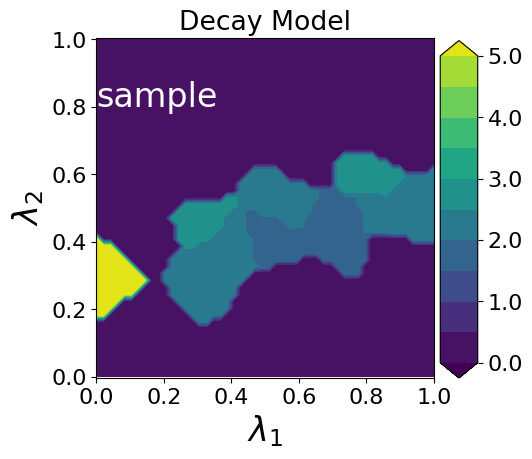
\includegraphics[width=\linewidth]{examples/fig_decay_q2/DecayModel--sample_N50_mc.png}
\end{minipage}
\caption{Observation taken at $t=0.5$s. The inverse image of the reference measure for set-based (left) and sample-based (right) solutions for $\nsamps=50$ parameter samples.}
\label{fig:heatrod-sol-ex2}
\end{figure}


Observing earlier in time helps especially in reducing the (marginal) values for the initial condition $\param_2$, while the rate $\param_1$ is still to some degree able to take any values in its original domain.
Both solution types suffer from discretization error, as evidenced by the break in the contour structure.
By comparison to \ref{fig:heatrod-sol-ex1}, there is more more confidence in the solution (represented by the reduced support of the image).

However, at $\nsamps=50$, the sample--based approach struggles to assign uniform probability to different contour events.
This may suggest that in situations with very limited model evaluation budget and set-valued solutions involving uniform uncertainties in measurements, the set-valued approach may serve a useful purpose.
